\documentclass[12pt,letterpaper]{article}
\usepackage{pdfpages}
\usepackage{fancyhdr}
\usepackage[colorlinks=true, urlcolor=blue, linkcolor=blue]{hyperref}
\usepackage{graphicx}
\usepackage[top=1.4in, left=0.5in, right=0.5in, bottom=0.8in]{geometry}
\usepackage[T1]{fontenc}
\usepackage{helvet}
\pagestyle{fancy}
\renewcommand{\headrulewidth}{0pt}
\renewcommand{\footrulewidth}{0pt}
\setlength{\parindent}{0em}
\setlength{\parskip}{1em}


\fancyfoot[C]{\setlength{\unitlength}{1in}\begin{picture}(5,0)\put(-1.8,-1){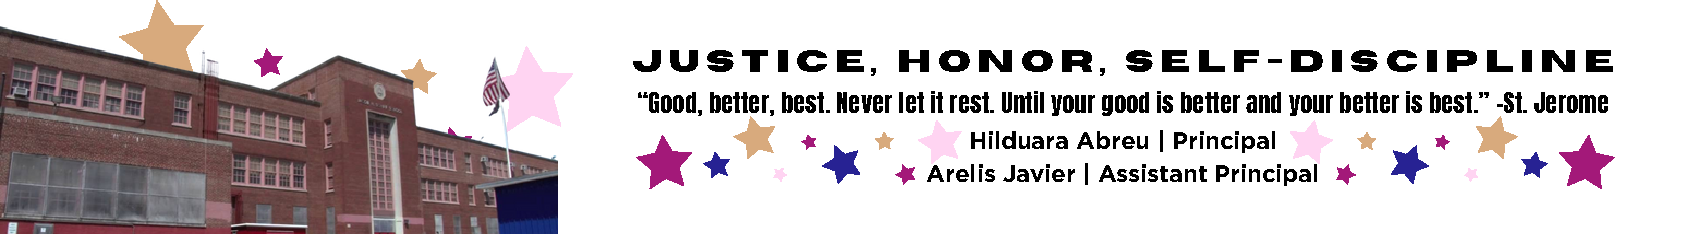
\includegraphics[width=8.8in,height=1.3in]{logo-1}}\end{picture}}
\fancyhead[C]{\setlength{\unitlength}{1in}\begin{picture}(5,0)\put(-1.9,-1){
\includegraphics[width=8.9in,height=1.3in]{logo-2}}\end{picture}}

\pagenumbering{gobble}
\addtolength{\evensidemargin}{-2in}
\addtolength{\topmargin}{-0.5in}
\addtolength{\textwidth}{0in}
%%%%%%%%%%%%%%%%%%%%%%%%%%%%%%%%%%%%%%%%%%%%%%%%%%%%%%%%%%%%%%%%%%

\begin{document}
\vspace*{0.5in}
Date: \href{https://www.ps192.org/apps/bbmessages/show_bbm.jsp?REC_ID=139439}{September 14, 2023} 

\textbf{Asunto: Política de uniforme escolar para P.S. 192}

Queridos padres y guardianes,

Esperamos que este mensaje los encuentre a ustedes y a sus familias con buena salud y buen humor. Mientras nos embarcamos en una nueva
año académico en P.S. 192, nos gustaría aprovechar esta oportunidad para informarle sobre la política de uniformes de nuestra escuela.
y enfatizar su importancia para fomentar una comunidad escolar positiva y cohesiva.

En P.D. 192, creemos que un código de vestimenta uniforme promueve un sentido de pertenencia, igualdad y un aprendizaje enfocado.
ambiente. A partir del curso académico 2023-2024, el uniforme de todos los alumnos consistirá en lo siguiente:
\begin{itemize}
	\item Camisa Borgoña: Se requiere que todos los estudiantes usen una camisa color burdeos como parte superior de
su uniforme.
	\item Pantalón azul marino: Pantalón o pantalón azul marino se utilizará como parte inferior del uniforme.
\end{itemize}
La política de uniforme se promoverá durante el horario escolar y en todos los eventos y actividades relacionados con la escuela, como
excursiones y asambleas especiales.

Los uniformes sirven como un elemento unificador dentro de nuestra comunidad escolar y ofrecen varias ventajas importantes:
		\begin{itemize}
		\item Promoción de la igualdad: los uniformes eliminan las disparidades socioeconómicas entre los estudiantes, asegurando que todos vistan de la misma manera, independientemente de las circunstancias financieras de su familia.
		\item Mejorar el enfoque: el uso de uniformes reduce las distracciones relacionadas con la moda y la presión de los compañeros, lo que permite a los estudiantes concentrarse en sus estudios y crecimiento personal.
		\item Fomentar el orgullo escolar: un uniforme inculca un sentido de orgullo y pertenencia entre los estudiantes, ayudando se identifican y aprecian a su comunidad escolar.
		\item Mejora de la seguridad: Los uniformes facilitan la identificación de intrusos en las instalaciones escolares, mejorando seguridad general.
		\item Prepararse para el éxito futuro: fomentar un código de vestimenta similar al atuendo profesional ayuda preparar a los estudiantes para futuras carreras donde una apariencia profesional es importante.
		\end{itemize}
\pagebreak
\vspace*{1.5cm}
Entendemos que la expresión personal es importante y, por lo tanto, ocasionalmente se programarán "Días de vestimenta informal" durante el año escolar, lo que permitirá estudiantes a expresar su individualidad a través de la elección de ropa.

Le solicitamos amablemente su cooperación y apoyo para garantizar que su hijo
Llega a la escuela vestido de acuerdo con nuestra política de uniforme. Creemos que Esto contribuirá a un ambiente de aprendizaje más positivo y productivo para
todos los estudiantes.

Si tiene alguna pregunta o inquietud sobre la política de uniformes, por favor
no dude en comunicarse con nuestra coordinadora de padres, Sra. Ángela Rijo:
\url{www.ps192.org/angela}, grupo de Whatsapp, ClassDojo, teléfono: (212) 775-9560, o en persona durante el horario de oficina de 9:00 a. m. a 3:00 p. m. Estamos aquí para ayudarle y apoyarle.

Gracias por su colaboración para fomentar una comunidad de aprendizaje sólida y vibrante en P.S. 192. Esperamos que el próximo año académico sea exitoso y enriquecedor.


En unidad,


\includegraphics[width=0.2\textwidth]{hil_signature}

\textbf{Hilduara Abreu}

\textbf{Principal}

\textit{La escuela donde el aprendizaje es divertido!}

\url{www.ps192.org}

\end{document}
